\documentclass{article}
\usepackage[utf8]{inputenc}
\usepackage{amssymb}
\usepackage{amsmath}
\usepackage{float}
\usepackage{epstopdf}
\usepackage{moreverb}
\usepackage{multicol}
\usepackage{listings}
\usepackage{mathrsfs}
\usepackage{graphicx}
\usepackage{cite}
\usepackage{tabularx}
\usepackage{listings}
\usepackage{subcaption}
\newcommand{\R}{\mathbb{R}}
\newcommand{\overbar}[1]{\mkern 1.5mu\overline{\mkern-1.5mu#1\mkern-1.5mu}\mkern 1.5mu}




\bibliographystyle{plain}
\title{APPM 5720 Homework 3}
\author{Wil Boshell, Fortino Garcia, Alex Rybchuk, Parth Thakkar}
\date{February 12, 2018}


\begin{document}

\maketitle

\maketitle

\section{Preliminaries}
Consider a grid with $N +1$ grid points $x_L = x_0 < x_1 < x_2 < \dots < x_N = x_R$, defining $N$ elements $\Omega_i =  \{x \in [ x_{i-1}, x_i ] \} $, $i=1,\dots,N$. We seek to approximate a function $f(x)$ on $x \in \left[ x_L, x_R \right]$ by $L_2$ projection onto the space of element-wise Legendre polynomials of degree $q$. This approximation takes the form 

  \begin{align*}
    \int_{\Omega_i} P_l(r) \sum_{k=0}^q c(k,i) P_k(r) \, dx = \int_{\Omega_i} P_l(r) f(x) \, dx, \quad l=0,\dots,q.
  \end{align*} 
where $c(i,k)$ are the coefficients of the $L_2$ projection. Here $r \in [-1,1]$ is a local variable such that on element $\Omega_i$ the affine map satisfies $x(-1) = x_{i-1}, x(1) = x_i$. This affine map (explicitly) is 

  \begin{align*}
    x(r) = \frac{1}{2}\left( \left(x_i - x_{i-1}\right) r + \left(x_i + x_{i-1}\right)\right) \implies dx(r) = \frac{1}{2}\left( x_i - x_{i-1}\right) dr.
  \end{align*}

\noindent Since the Legendre polynomials are orthogonal with respect to the weight functions $w(x) = 1$ and 
  \begin{align*}
    \int_{-1}^1 P_l(x)P_n(x) \, dx = \frac{2}{2n + 1} \delta_{l,n},
  \end{align*}
the above system of equations reduces to

  \begin{align*}
    \int_{\Omega_i} P_l(r) \sum_{k=0}^q c(k,i) P_k(r) \, dx & = \sum_{k=0}^q c(k,i) \int_{\Omega_i} P_l(r) P_k(r) \, dx \\
    & = \sum_{k=0}^q \frac{1}{2} c(k,i) \left( x_i - x_{i-1}\right) \int_{-1}^1 P_l(r) P_k(r) \, dr \\
    & = \frac{1}{2} c(l,i) \left( x_i - x_{i-1}\right) \frac{2}{2l + 1}.
  \end{align*}
On the right hand side of our formulation, we approximate this using the Gauss-Lobato-Legendre weights and nodes $w_j, \, r_j$ to obtain

  \begin{align*}
    \int_{\Omega_i} P_l(r) f(x) \, dx = \frac{1}{2} \left( x_i - x_{i-1}\right) \int_{-1}^1 P_l(r) f(x(r)) \, dr \approx \frac{1}{2} \left( x_i - x_{i-1}\right)\sum_{j=0}^q w_j P_l(r_j) f(x(r_j)).
  \end{align*}
We note that both sides have $\frac{1}{2} \left( x_i - x_{i-1}\right)$ so that our system of equations reduces to 

  \begin{align*}
    c(l,i) \frac{2}{2l + 1} = \sum_{j=0}^q w_j P_l(r_j) f(x(r_j)) \implies c(l,i) = \frac{2l + 1}{2} \sum_{j=0}^q w_j P_l(r_j) f(x(r_j)), \quad l = 0,\dots, q .
  \end{align*}
That is, the set of $N$ decoupled linear systems of equations of size $(q+1)\times(q+1)$ forms a diagonal matrix which can easily be solved without calling a routine that performs Gaussian elimination.

\section{Increasing Element Count}
We begin by considering a set of functions $f(x)$ and showing that with $q=1,2,\dots,$ the approximation described above is increasingly accurate with an increasing number of elements as measured in the uniform and $L_2$ norm. In the following plots, note that $q = 1$ is in red and increasing $q$ is colored according to the usual ordering of the color spectrum (i.e. ROYGBV applies).

\subsection{Smooth, Infinitely Differentiable Function}
Let us first consider the function
  \begin{align*}
    f(x) = e^{\left( x - 2\right)^2}, \quad x\in \left[ 0,4\right].
  \end{align*}
We note that this function is continuous and infinitely differentiable, and so we expect that our approximation scheme should increase in accuracy as we increase $q$ and the number of elements. Indeed, this appears to be the case as demonstrated by the following plot of data. Consistently it appears that for a fixed number of elements an increase in $q$ decreases the error, and for fixed $q$ an increase in number of elements (i.e. smaller average element sizes) decreases the overall error as expected.
\begin{figure}[H]
  \centering
  \begin{minipage}{.6\textwidth}
    \centering
    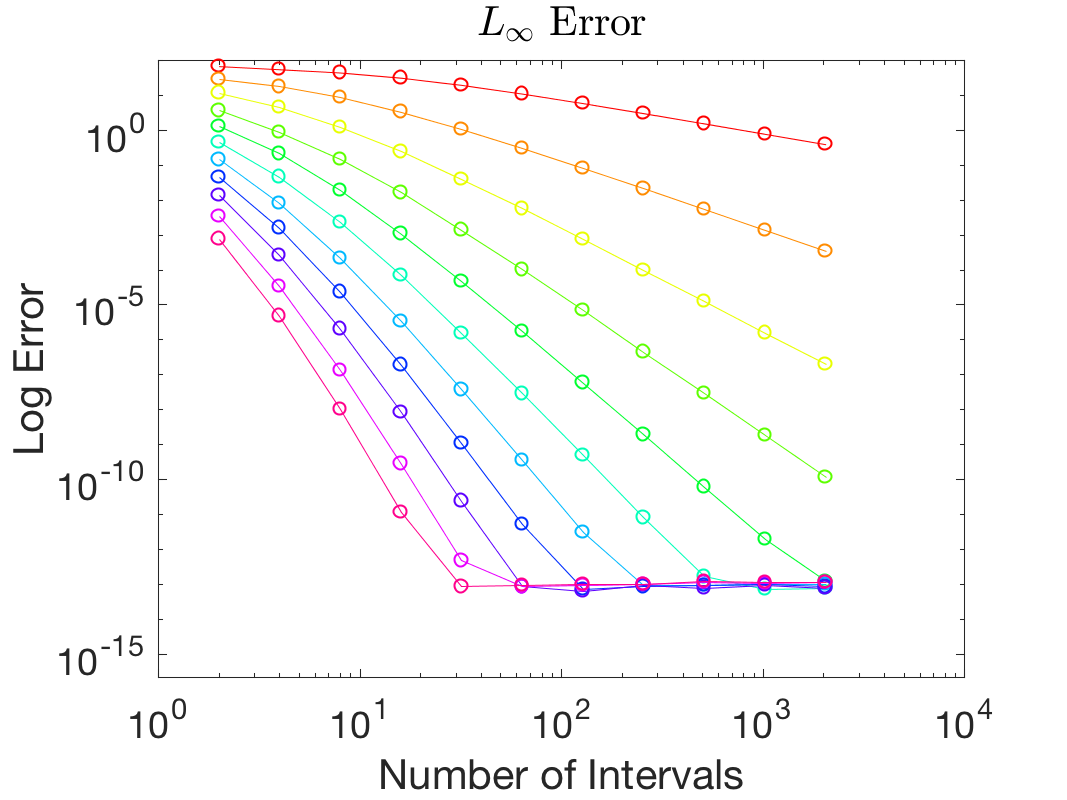
\includegraphics[width=\linewidth]{maxError_0.png}
    \captionof{figure}{Max Error for an Exponential}
    \label{fig:max0}
  \end{minipage}%
  \begin{minipage}{.6\textwidth}
    \centering
    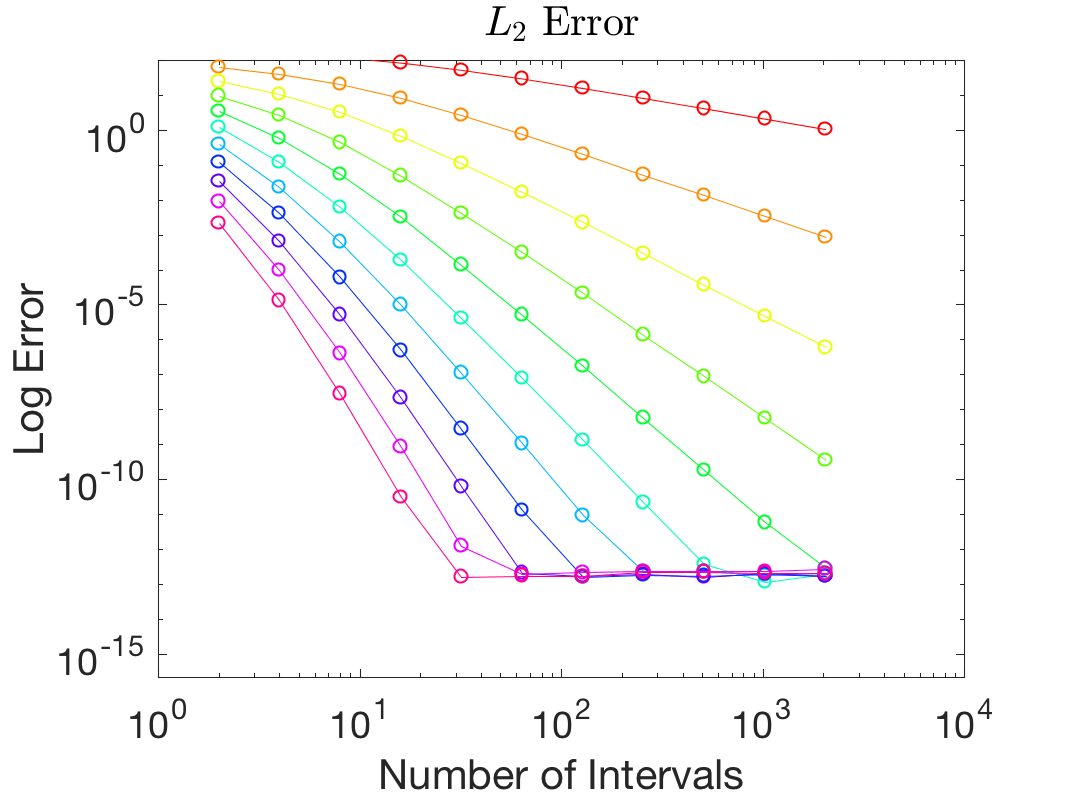
\includegraphics[width=\linewidth]{squareError_0.png}
    \captionof{figure}{$L_2$ Error for an Exponential}
    \label{fig:square0}
  \end{minipage}%
\end{figure}

\noindent The situation is much the same with respect to the $L_2$ error as depicted above in the right panel. We see that the $L_2$ error doesn't reach machine precision and is slightly worse compared to the uniform error. \newline


\subsection{Smooth, Infinitely Differentiable, Periodic Function}
\noindent We move on to another infinitely differentiable function, this time to the periodic function

  \begin{align*}
    f(x) = \sin x , \quad x \in \left[ -\pi, \pi\right].
  \end{align*}
Below is a plot of the error.

\begin{figure}[H]
  \centering
  \begin{minipage}{.6\textwidth}
    \centering
    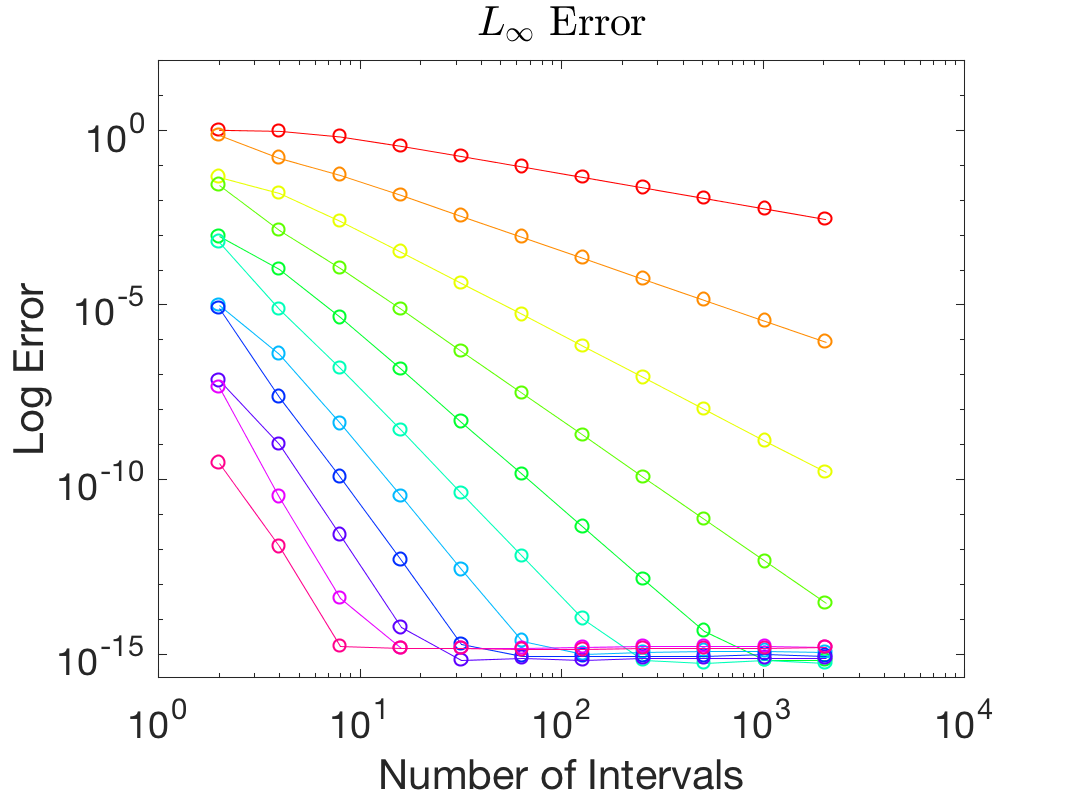
\includegraphics[width=\linewidth]{maxError_2.png}
    \captionof{figure}{Max Error for $\sin x$}
    \label{fig:max2}
  \end{minipage}%
  \begin{minipage}{.6\textwidth}
    \centering
    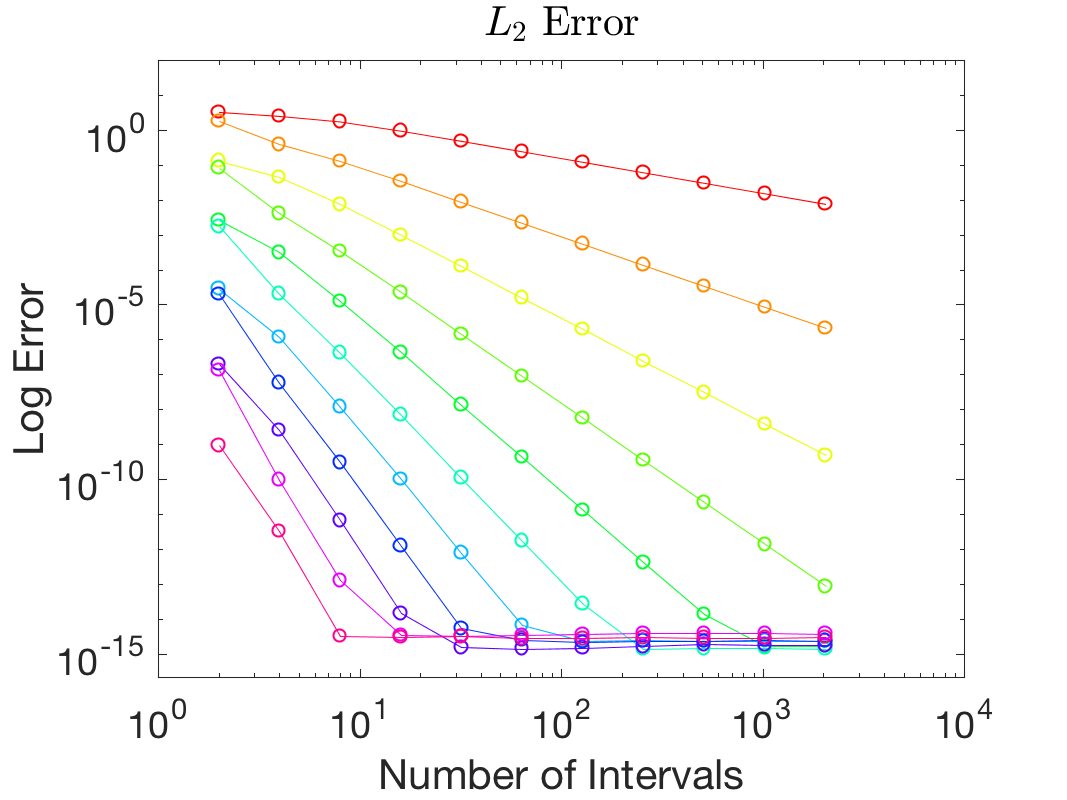
\includegraphics[width=\linewidth]{squareError_2.png}
    \captionof{figure}{$L_2$ Error for $\sin x$}
    \label{fig:square2}
  \end{minipage}%
\end{figure}


\noindent As before, the $L_\infty$ error for each $q$ is better than that of the $L_2$ error and decreases with increasing number of intervals used to build our approximation. One curiosity here is that it appears that choosing a slightly smaller $q$ and increasing the number of intervals outperforms large $q$ values past around $100$ intervals. \newline

\subsection{Continuous, Non-Differentiable Function}
\noindent So far we have only considered smooth, differentiable functions. Let us now examine a case of a continuous function that is not continuously differentiable, 

\begin{align*}
  f(x) = | x | , \quad x \in [-2,2].
\end{align*}

\noindent We might expect that the error away from the non-differentiable point $x = 0$ to be incredibly low since away from $x = 0$ the function is linear and for $q \geq 2$ we expect to approximate the function exactly (since choosing a quadrature with $n$ nodes gives us accurate integration of polynomials of degree up to $2n - 3$ for Gauss-Lobato nodes). However, since $x = 0$ is in the region of interest, the error of approximating near the problem point will dominate the overall error in approximating the function globally. 

\begin{figure}[H]
  \centering
  \begin{minipage}{.6\textwidth}
    \centering
    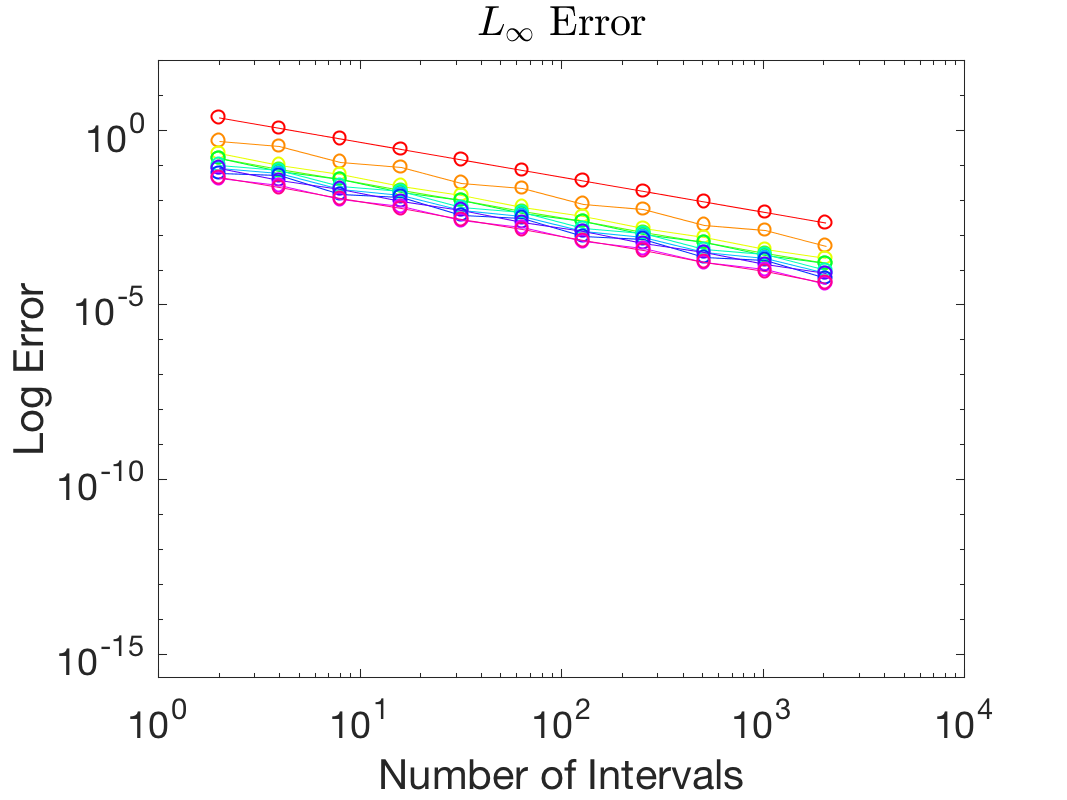
\includegraphics[width=\linewidth]{maxError_1.png}
    \captionof{figure}{Max Error for $|x|$}
    \label{fig:max1}
  \end{minipage}%
  \begin{minipage}{.6\textwidth}
    \centering
    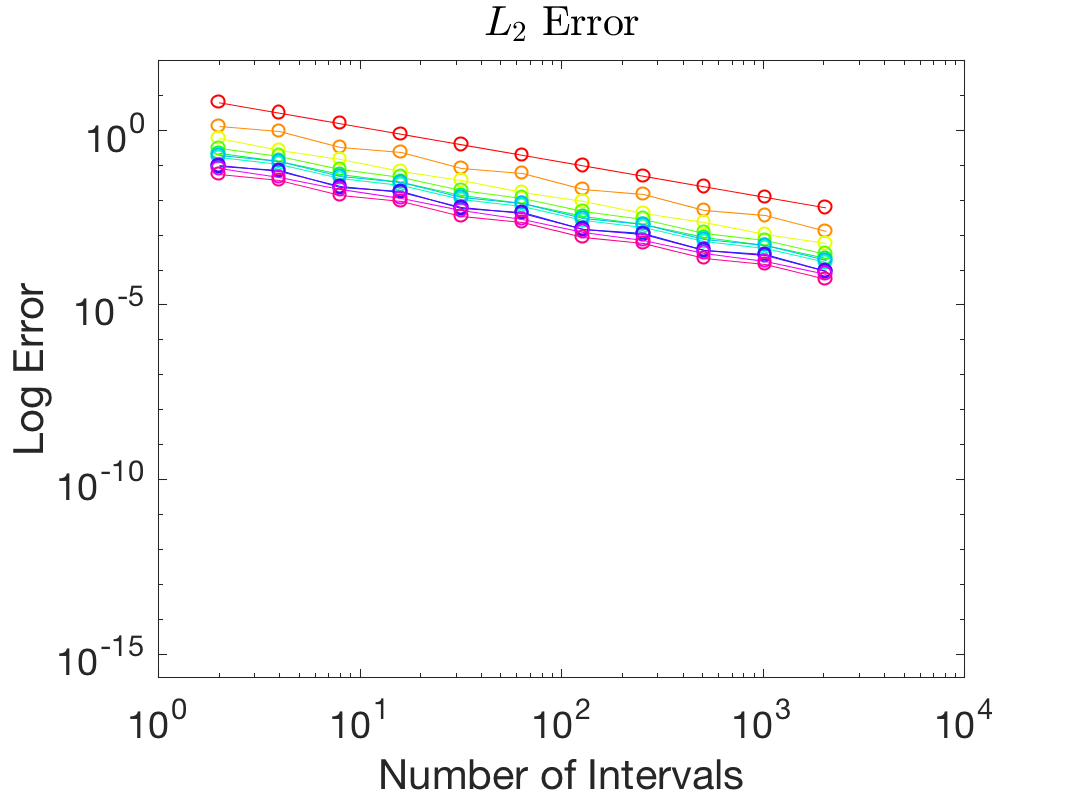
\includegraphics[width=\linewidth]{squareError_1.png}
    \captionof{figure}{$L_2$ Error for $|x|$}
    \label{fig:square1}
  \end{minipage}%
\end{figure}

\noindent The above error plot shows that, as before, increasing $q$ and number of intervals used does decrease the overall error (and the $L_\infty$ error is better than the $L_2$ error). In this case, however, we make few gains and don't achieve more than $5$ digits of accuracy. The given formulation then is problematic for functions that are non-differentiable, even for a function that is not differentiable at a single point.

\section{Increasing Polynomial Degree}
The relationship between error and an increase in Legendre polynomial degree was explored. The function $\sin(x)$ was chosen for this case study. In order to investigate whether the error followed a trend like $c^{-q}$, we plotted $\log\big[max(||E||_{2})\big]$ vs $\log(q)$ where E is the error and q is the highest degree of polynomials. This was done for total number of intervals = $5,6,7,8,9$ and $10$.
\begin{figure}[H]
  \centering
  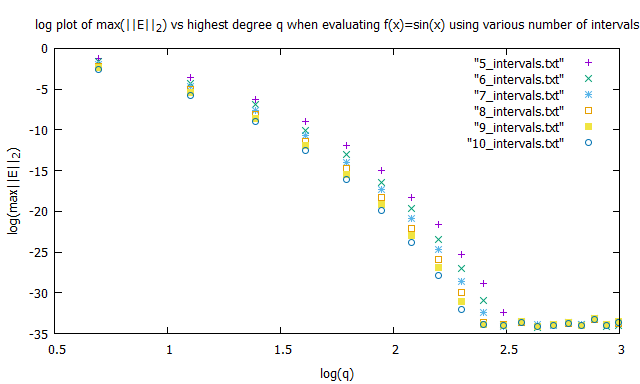
\includegraphics[scale=0.5]{hw3.png}
  \caption{Plot of Increasing Legendre degree $q$ for Fixed Number of Intervals}
  \label{fig:incDegree}
\end{figure}
\noindent We can see that we almost get a straight line with negative slope (starting with q=4) up to a certain value of $q$ on the log-log plot. This means that the error does obey the law $E=c^{-q}$. After a certain value, the error is nearly constant, i.e. the value of log$\big[max(||E||_{2})\big]$ goes down to $-35$. This is because the error $E=e^{-35}$ is of the order of $10^{-16}$, which is machine precision, i.e. it is beyond measure by our computers which work on double precision.

\section{Exploring Curiosities}
\subsection{Discontinuous, Non-Differentiable Function}
Let us consider the following function
\begin{align*}
	f(x) = \left\{ \begin{array}{cc} 
                1 & \hspace{5mm} x \ge 0 \\
                -1 & \hspace{5mm} x < 0 
                \end{array} \right.
\end{align*}
We note that this function is not differentiable in the usual sense, nor is it even continuous. We then expect the prescribed approximation method to break down due to the jump discontinuity. 
\begin{figure}[H]
  \centering
  \begin{minipage}{.6\textwidth}
    \centering
    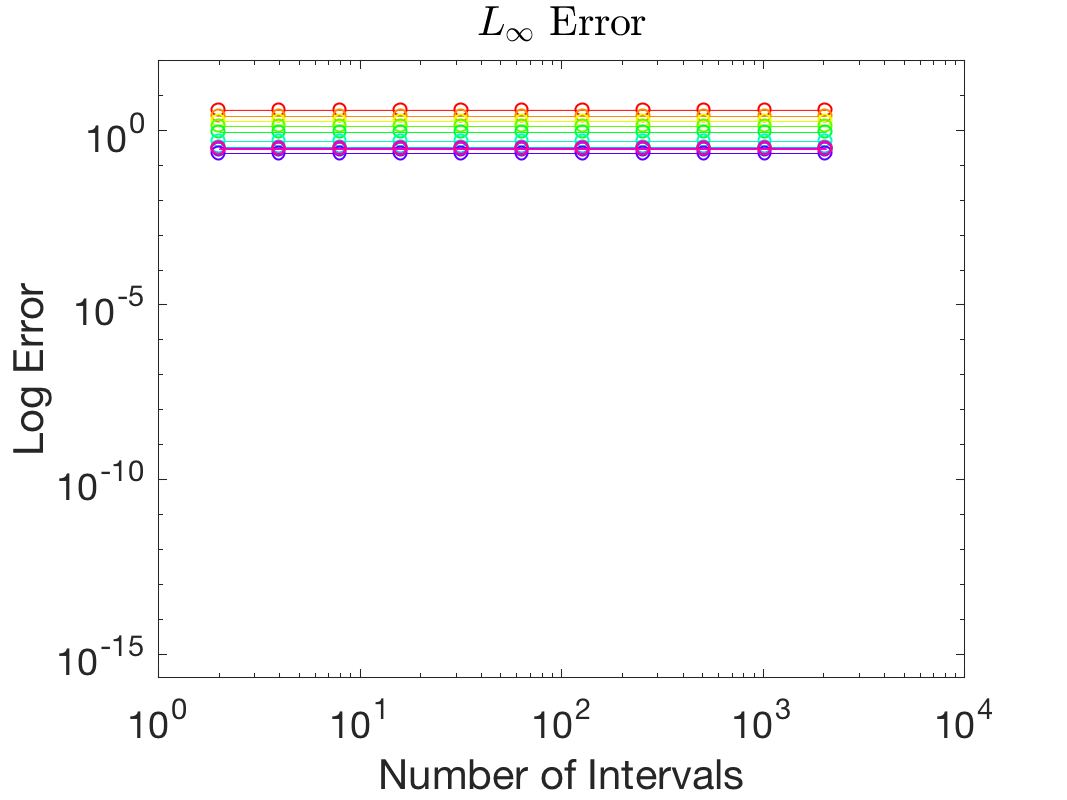
\includegraphics[width=\linewidth]{maxError_3.png}
    \captionof{figure}{Max Error for $Sgn(x)$}
    \label{fig:max3}
  \end{minipage}%
  \begin{minipage}{.6\textwidth}
    \centering
    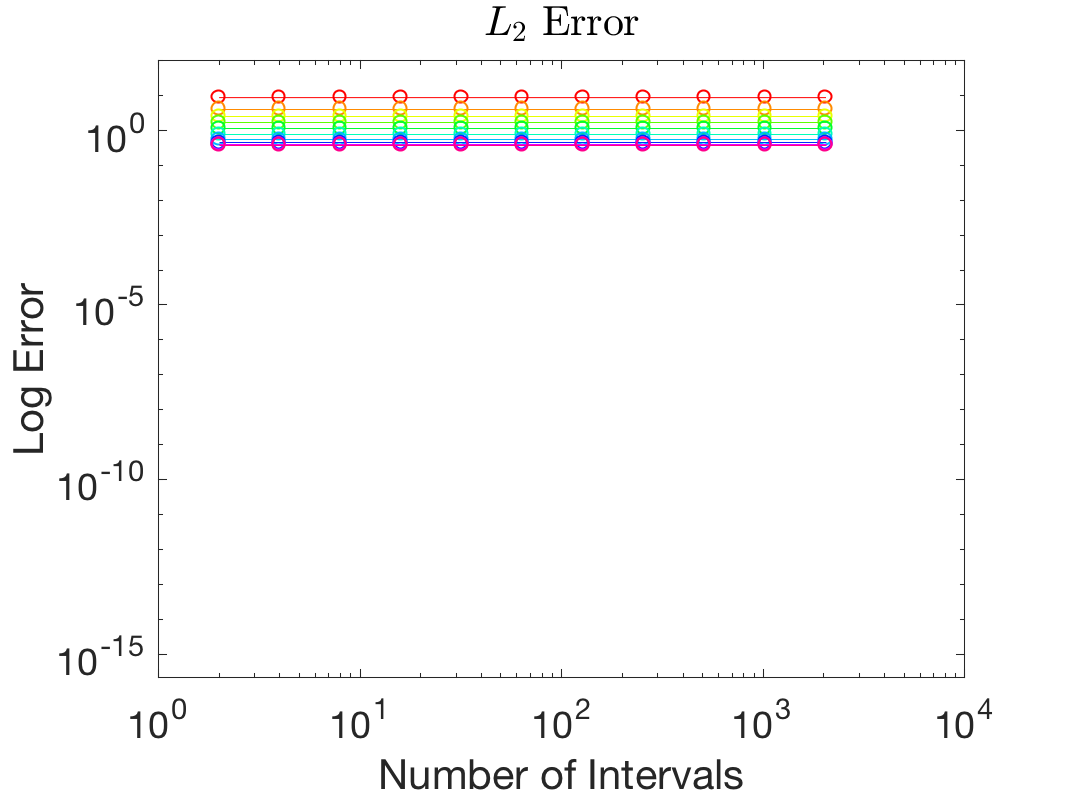
\includegraphics[width=\linewidth]{squareError_3.png}
    \captionof{figure}{$L_2$ Error for $Sgn(x)$}
    \label{fig:square3}
  \end{minipage}%
\end{figure}
\noindent Interestingly, the error does not decrease with increasing number of intervals used in our approximation. This suggests that the jump discontinuity cannot be well approximated by our method. As before, increasing $q$ in general does decrease the overall error, but no more than a single digit of accuracy is attained for $q \leq 20$. 

\subsection{Using Chebyshev Polynomials / Monomials as Basis Functions}
Let a function $f(x)$ be approximated by using Chebyshev polynomials up to degree $q$. Let the grid comprise of intervals $\Omega_{i}$. The function $f(x)$ would have a representation
\begin{align*}
    f(x) = \sum_{k=0}^{q} c(k,i) T_{k}(r_{i}(x)), \quad x \in \Omega_{i},
\end{align*}
where $r_{i}(x)$ be the linear mapping from $x \in \Omega_{i}$ to $r_{i} \in [-1,1]$. Thus, we would have
\begin{align*}
    \int_{\Omega_{i}} \frac{f(x) T_{l}(r_{i}(x)}{\sqrt{1 - (r_{i}(x))^{2}}} dx = \int_{\Omega_{i}} \sum_{k=0}^{q} c(k,i) \frac{T_{k}(r_{i}(x)) T_{l}(r_{i}(x))}{\sqrt{1 - (r_{i}(x))^{2}}} dx = c(l,i).
\end{align*}
The utility in using Chebyshev polynomials approximation is that the Chebyshev polynomails give the best approximation to a continuous function under the maximum norm. In addition, the roots of the Chebyshev polynomials have an explicit formula so that building quadratures with the Chebyshev polynomials would be efficient. \newline

\noindent If we use the monomial basis functions, i.e. \{$1, x, x^{2}, \cdots x^{q}$\} then the function $f(x)$ would be represented as 
\begin{align*}
    f(x) =  \sum_{k=0}^{q} c(k,i) x^{k}, \quad x \in \Omega_{i}.
\end{align*}
In general, this will yield a dense Vandermonde matrix which will require the use of a solver (i.e. \verb|LAPACK|) to find the coefficients. On the interval $[0,1]$, this creates the Hilbert matrix which is ill-conditioned and singular to working precision for small maximum degree $q$. \newline

\subsection{Perturbing Uniform Grid Spacing}

The effect of grid spacing on approximation error was explored. The function $\sin(x)$ was approximated on the interval $[0,3]$. A grid with uniform spacing was intially created. Then it was purturbed with noise sampled from a uniform distribution. The magnitude of the noise was varied between $0\%$ and $30\%$ of the length of the domain. Error was observed to increase as purturbation magnitude increased. 

\begin{figure}[H]
  \centering
  \begin{minipage}{.6\textwidth}
    \centering
    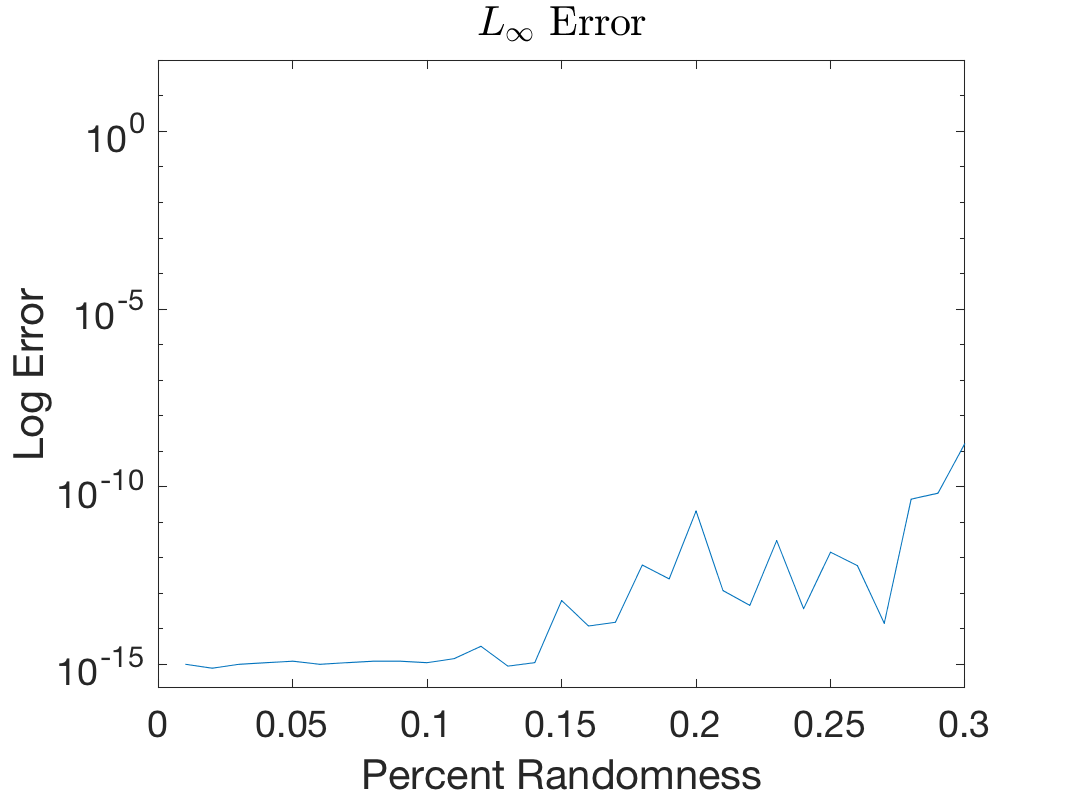
\includegraphics[width=\linewidth]{maxRandErr.png}
    \captionof{figure}{Max Error as Noise Increases}
    \label{fig:max3}
  \end{minipage}%
  \begin{minipage}{.6\textwidth}
    \centering
    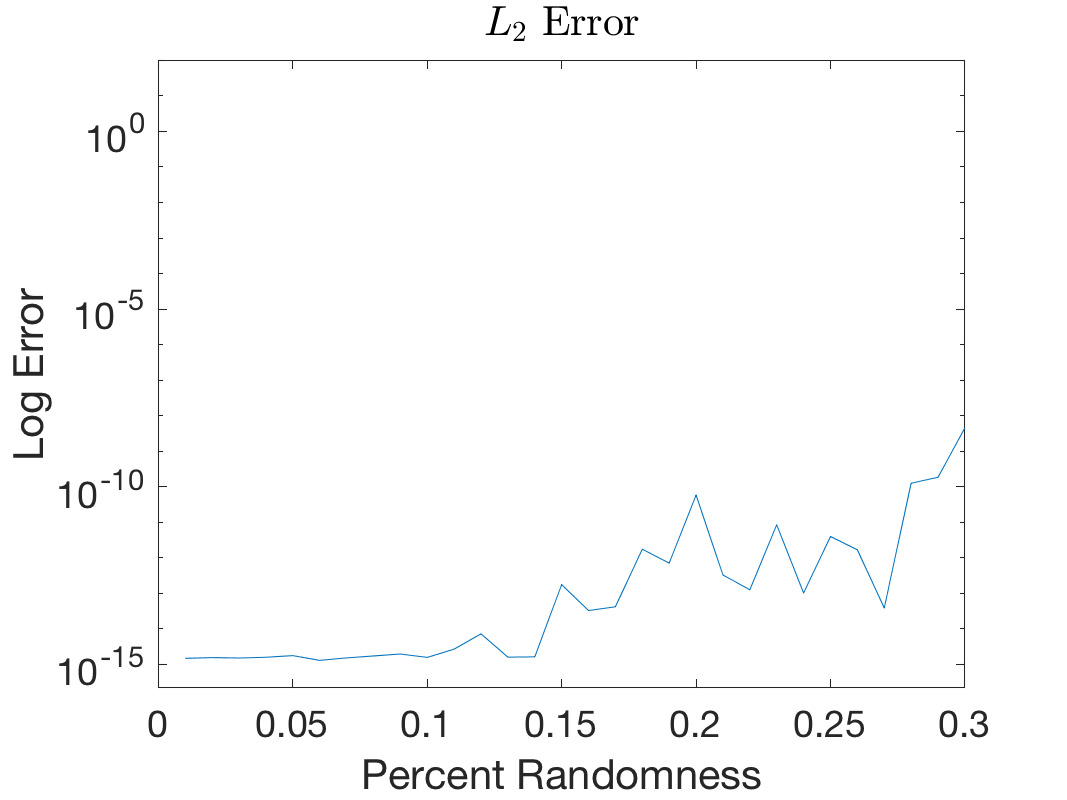
\includegraphics[width=\linewidth]{squareRandErr.png}
    \captionof{figure}{$L_2$ Error as Noise Increases}
    \label{fig:square3}
  \end{minipage}%
\end{figure}

\end{document}
